\documentclass[9pt]{beamer}
\usepackage{algorithm,algorithmic}
\usepackage{amsmath}
\usepackage{amssymb}
\usepackage{proof,mathpartir}
\usepackage{eqparbox}
\usepackage{siunitx,amsmath}
%meiksens
\newcommand{\itemEq}[1]{%
	\begingroup%
	\setlength{\abovedisplayskip}{0pt}%
	\setlength{\belowdisplayskip}{0pt}%
	\parbox[c]{\linewidth}{\begin{flalign}#1&&\end{flalign}}%
	\endgroup}
\renewcommand\algorithmiccomment[1]{%
	\hfill\#\ \eqparbox{COMMENT}{#1}%
}
% Encoding
\usepackage[T1]{fontenc}
% UTF8 input
\usepackage[utf8]{inputenc}
% Use german language
\usepackage[english]{babel}

% Use the given theme
\usetheme{HLISP}
\renewcommand{\algorithmicforall}{\textbf{foreach}}
\title{Seminar on Computational Contracting Approaches:\\
J\o{}rgensen's Dilemma }
\author[]{Karam Kharraz}


\subject{Beispiel}
\keywords{example, beamer template}

% Use TikZ
\usepackage{tikz}
\tikzstyle{node} = [shape=circle,draw,fill=uzlmain!20,inner sep=2pt, minimum width=4pt]
\tikzstyle{box} = [shape=rectangle,draw,fill=uzlmain!20,inner sep=2pt,minimum width=3cm,minimum height=1cm]

\begin{document}
	
\frame{\titlepage}
	




\begin{frame}
\frametitle{Outline}
\begin{itemize}
	\item Introduction
	\item Problem Definition: J\o{}rgensen's Dilemma
	\item Proposed solution: I/O Logic
	\item Evaluation
	\item Conclusion
\end{itemize}
\end{frame}

\begin{frame}
\frametitle{Classification of Problems: Paper to be studied}
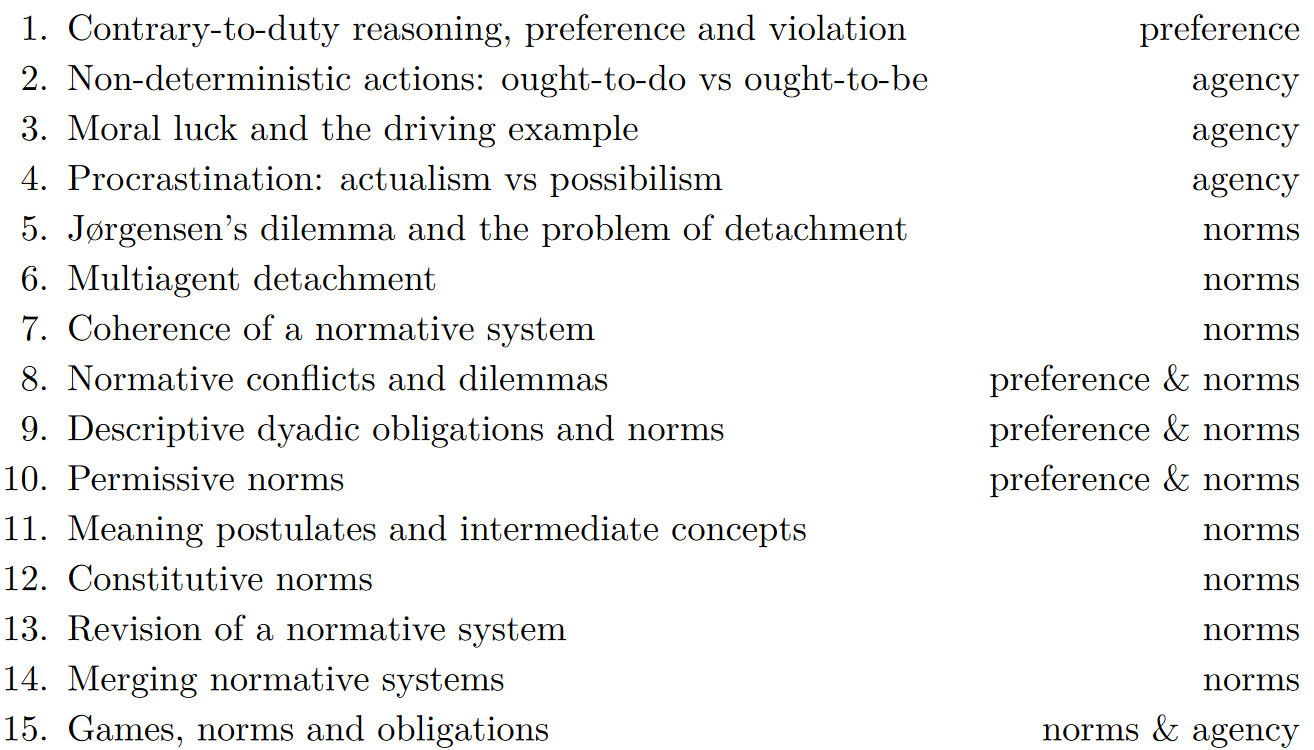
\includegraphics[scale=0.55]{class.png}
\end{frame}

\begin{frame}
\frametitle{Imperative and logic}
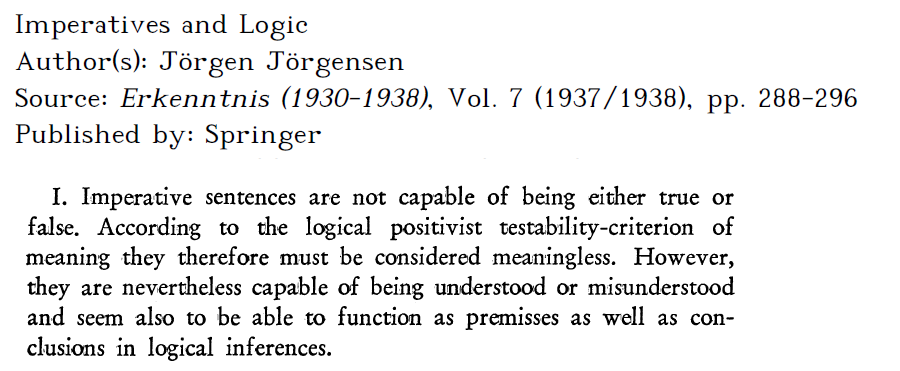
\includegraphics[scale=0.50]{jorgensen.png}
\end{frame}


\begin{frame}
\frametitle{Standard deontic Logic:1951}
\centering
\includegraphics[scale=0.60]{sdl.png}
\end{frame}



\begin{frame}
\frametitle{Deontic logic: Axioms for Standard Deontic Logic \cite{von1951deontic} (System KD) }
Set of axioms and inference rules to reason about a system of norms:
\begin{enumerate}
	\item Taut: All  tautologies From Propositional logic are wffs\footnote[frame]{Well formed formulas} of the language.
	\item  Axiom K: $O(p\rightarrow q)\rightarrow (O(p) \rightarrow O(q))$ 
	\item  Axiom D: $O(p)\rightarrow \lnot O(\lnot p)$
	\item Modus Ponens: \\$ ~~~~~~~~~~~~~~~~~~~~~~~~~~\inferrule*[left=MP]{\vdash p \rightarrow q ~~~~~~~~~~ \vdash p}{\vdash q}$
	\item Necessity: \\$~~~~~~~~~~~~~~~~~~~~~~~~~~~~\inferrule*[left=Nec]
	{\vdash p}{\vdash O(p)}$ 
	
\end{enumerate}	
\end{frame}

\begin{frame}
\frametitle{Tautologies in Propositional logic}
\centering
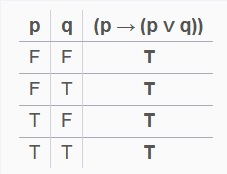
\includegraphics[scale=0.60]{table.jpg}
\begin{itemize}
	\item $p \rightarrow (p \vee q)$ is a tautology.
	\item In SDL using Necessity + K we get:\\
	$O(p)\rightarrow O(p \vee q)$
\end{itemize}
\end{frame}
\begin{frame}
\frametitle{Contrary to duty paradox caused by J\o{}rgensen's Dilemma?}
\begin{enumerate}
	\item It is forbidden kill. $O(\lnot kill)$
	\item If one ever kills he must kill gently. $\color{red}{kill} \rightarrow O(killgently)$.
	\item Someone just killed. $kill$
	\item $killgenly \rightarrow kill$ (Common sense) 
\end{enumerate}	

by assuming the set 
\begin{itemize}
	\item from (2) and (3) By MP : $O(kill gently)$
	\item we know that $kill gently \rightarrow kill$.
	\item by NEC we get $O(kill gently \rightarrow kill)$ 
	\item by Axiom K: $O(kill gently \rightarrow kill) \rightarrow (O(kill gently) \rightarrow O(kill) )$
	\item by MP and Axiom D: we conclude: $\lnot(O(\lnot kill))$ (4) 
	\item by (1) and (4) we have $O(\lnot kill) \wedge \lnot O(\lnot kill) $ \textbf{Paradox (Gentle Murderer)} 
\end{itemize}	
\end{frame}

\begin{frame}{Wrap up}
\begin{itemize}
\item The J\o{}rgensen's Trilemma could be understood as follows:
\begin{enumerate}
	\item Logical inference requires that the elements have truth-values.
	\item Normative statements do not have truth-values.
	\item There are logical inferences between normative statements.
\end{enumerate}
\item Proposed solution: \textit{Input/Output logic}
\end{itemize}
\end{frame}

\begin{frame}{What is I/O Logic}
	\begin{itemize}
	\item I/O logic is a non classical logic.
	\item Reason about a set $G$ of norms.
	\item Norms are pairs (a,x), where a and x are boolean formulae.
	\item $a$ is called an input, while $x$ is the corresponding output.
	\item The question is: What is the right output for a situation  $A$ a set of boolean formulae.
	\end{itemize}
    \end{frame}

\begin{frame}{What should I do ? $Out_x(G,A)$}
\centering
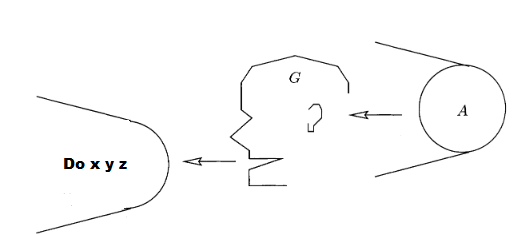
\includegraphics[scale=0.60]{react.png}
\end{frame}


\begin{frame}{Basic operations: Consequence}
\begin{definition}[Consequence Cn(A)]
	$Cn(A)$ denotes the set of logical consequences of $A$ in classical propositional logic.It returns the set of all provable propositional formulae provable assuming the fact in $A$\\
	$Cn(a)=\{x~|~A\vdash x \}$
\end{definition}
\begin{example}
	\begin{itemize}
\item $A_1= \{x,y\}$ then $Cn(A)= \{x, y, x \vee y, x \wedge y \vee \dots \}$
\end{itemize}
\end{example}
\end{frame}

\begin{frame}{Basic operations: Image of a $A$}
\begin{definition}[G(A)]
	$G(A)$ is the set of answers of a set of inputs.\\
	$G(a)=\{x~|~(x,a). x \in G \wedge a \in A  \}$
\end{definition}
\begin{example}
	\begin{itemize}
		\item $G_1=\{(a_1,x_1),(a_2,x_2)\} $ and $A_1\{a_1,z\} $ and $A_2=\{a_1,a_2,x_2\}$
		\item $G_1(A_1)= \{x_1\}$
		\item $G_1(A_2)= \{x_1,x_2\}$
	\end{itemize}
\end{example}
\end{frame}






\begin{frame}
\frametitle{Derivable Properties }

	
	$ ~~~~~~~~~~~~~~~~~~~~~~~~~~\inferrule*[left=$\top$]{--}{\top,\top}$
	$~~~~~~~~~~~~~~~~~~~~~~~~~~~~\inferrule*[left=SI]
	{(a,x)~~~b \vdash a}{(b,x)}$ \\
	$ ~~~~~~~~~~~~~~~~~~~~~~~~~~\inferrule*[left=WO]{(a,x) ~~ x\vdash y}{(a,y)}$
	$ ~~~~~~~~~~~~~~~~~~~~\inferrule*[left=AND]{(a,x) ~~ (a,y)}{(a,x\wedge y)}$\\
	$ ~~~~~~~~~~~~~~~~~\inferrule*[left=OR]{(a,x) ~~ (b,x)}{(a\vee b,x)}$
	$ ~~~~~~~~~~~~~~~~~\inferrule*[left=CT]{(a,x) ~~ (a\wedge x,y)}{(a,y)}$
\pause
\centering
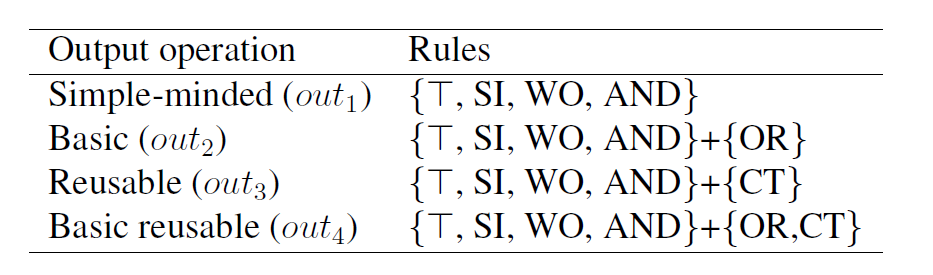
\includegraphics[scale=0.30]{out.png}
\end{frame}

\begin{frame}{Contrary to duty reasoning in I/O Logic}
\begin{definition}[Maximal non excessive subsets]
	$Maxfam(G,A,C)= H_{max} \subseteq G~.~out_x(H,A)$ is consistent. 
\end{definition}
\begin{definition}[Consistent out]
	$out_x^{\cap}(G,A)= \bigcap\{out_x (H,A) | H \in Maxfam(G,A,A)\} $
\end{definition}
\begin{example}[Gentle murderer]
	\begin{itemize}
	\item $G=\{(\top, \lnot kill), (kill, kill\_gently)\} $and $A=\{kill\}$
	\item We have $H\in out_1(G,A)=\{kill\_gently, \lnot kill\}$ inconsistent. because $\top$
    \item $H=\{kill\} \in out_1(G,A)$ and $Out(H,A) = kill\_gently$ is consistent
	\item $out_x^{\cap}(G,A)=kill\_gently$
	\end{itemize}
\end{example}
\end{frame}
\begin{frame}{Conclusion}
\centering
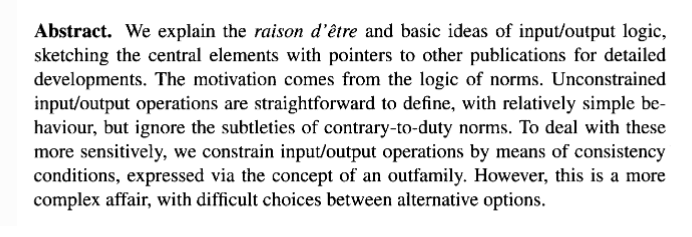
\includegraphics[scale=0.50]{conclusion.png}
\end{frame}

\end{document}










%\documentclass[xcolor=table]{beamer}
%\usepackage[linesnumbered,lined,boxed,commentsnumbered]{algorithm2e}
%\usepackage{algorithmic}
%\usepackage{float}
%\usepackage{amsmath}
%\usepackage{amssymb}
%% This is an example to show the beamer template HLISP.
%
%% Encoding
%\usepackage[T1]{fontenc}
%% UTF8 input
%\usepackage[utf8]{inputenc}
%% Use german language
%\usepackage[ngerman]{babel}
%
%% Use the given theme
%\usetheme{HLISP}
%
%\begin{document}
%
%\frametitle{OR61}
%
%\begin{frame}
%\frametitle{Outline}
%\begin{enumerate}
%	\item RoRo at LHG
%	 \begin{itemize}
%	 \item{Ro-Ro vs Container transportation}
%	 \item Baltic sea and LHG
%	 \end{itemize}
%	\item Scenario: Opportunistic Synchromodality
%	\begin{itemize}
%		\item Isolated Bookings.
%		\item Delayed Arrival possible consequences
%		\item Harbor notification 
%		\item Requirement: Negotiation of replanting
%	\end{itemize}
%	\item Model:
%	 \begin{itemize}
%	 	\item Booking model: Quality of delivery (Cost, Delay), chain effect
%	 	\item Timing modeling: planning and real execution
%	 	\item Game theory: Nash equilibrium vs Global optimization
%	 \end{itemize}
%	\item Decision procedure:
%	\begin{itemize}
%		\item Wait or replace?
%		\item How to replace?
%	\end{itemize} 
%
%	\item Conclusion:
%	\begin{itemize}
%		\item Effect of the procedure
%		\item Lack of information sharing 
%		 (Motivation for the architecture)
%	\end{itemize}
%\end{enumerate}
%\end{frame}
%
%
%
%\begin{frame}[fragile]
%\begin{algorithm}[H]
%	\begin{algorithmic}[1]
%		\FOR{$i=1$ to $N$}
%		\FOR{$j=1$ to $JJJJ$}
%		\STATE $energy[i*JJJ+j] =$ \\
%		$ interpolate(AAA[i*JJJ+j], ZZZ)$
%		\ENDFOR
%		\ENDFOR
%	\end{algorithmic}
%	\caption{pseudocode for the calculation of }
%	\label{alg:seq}
%\end{algorithm}
%\end{frame}	
%\end{document}
